\documentclass[11pt, oneside]{article} 
\usepackage{geometry}
\geometry{letterpaper} 
\usepackage{graphicx}
	
\usepackage{amssymb}
\usepackage{amsmath}
\usepackage{parskip}
\usepackage{color}
\usepackage{hyperref}

\graphicspath{{/Users/telliott_admin/Dropbox/Tex/png/}}
% \begin{center} 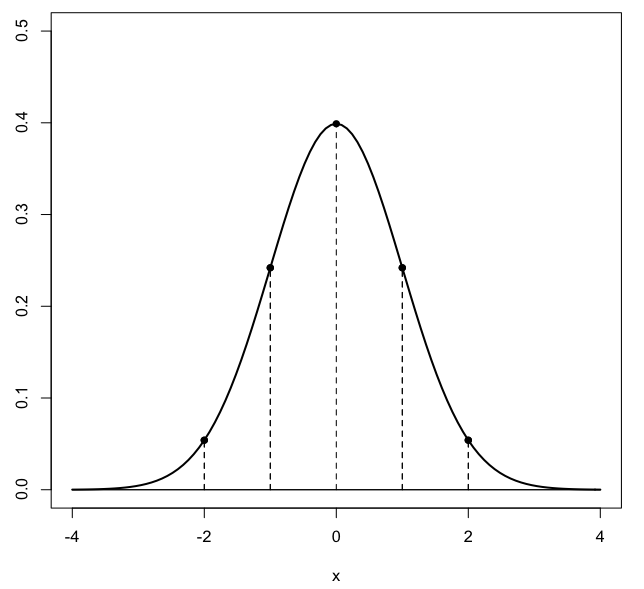
\includegraphics [scale=0.4] {gauss3.png} \end{center}

%break
\title{Shortest path}
\date{}

\begin{document}
\maketitle
\Large

\label{sec:Shortest_path}

As shown in the figure below, we have two points $P$ and $Q$, which might be, say, the origin and destination of a journey that must also go to the river (horizontal line at the top).  The point where we reach the river can be adjusted, and we seek the path that has the shortest overall distance.

\begin{center} 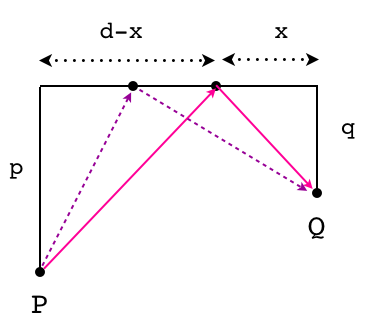
\includegraphics [scale=0.5] {short1.png} \end{center}

There is a hard way to do this problem, and an easy way.  The hard way involves a tiny bit of calculus (to do the minimization).  I'll show that one first.  

Depending on where we put the point on the river, we have a horizontal distance $x$ to that point from $Q$, and a horizontal distance $d-x$ to the same point from $P$.

The path consists of two parts, from $P$ to the river, and from the river back to $Q$.  That distance is

\[ \sqrt{p^2 + (d-x)^2} + \sqrt{q^2 + x^2} \]

We take the derivative with respect to $x$.  It's a little tricky.  

For the first term, we get the denominator from applying the power rule to the square root (plus a factor of $1/2$), then we apply the chain rule to $(d-x)^2$ and get $2(d-x)$ in the numerator, and finally a factor of $-1$ from $-x$.  The twos cancel.  The second term is similar.  

Set the result equal to $0$:
\[ - \frac{d-x}{\sqrt{p^2 + (d-x)^2}} +  \frac{x}{\sqrt{q^2 + x^2}} = 0 \]
\[ \frac{x}{\sqrt{q^2 + x^2}} = \frac{(d-x)}{\sqrt{p^2 + (d-x)^2}} \]

It's just algebra from this point.  But notice that we don't need it.  Both of these ratios correspond to the cosine of an angle.
\begin{center} 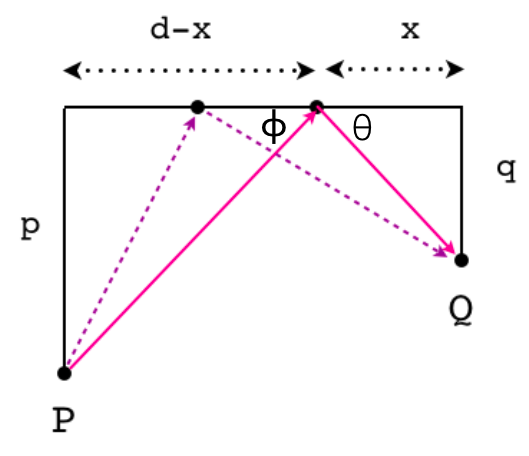
\includegraphics [scale=0.5] {short3.png} \end{center}

\[ \frac{x}{\sqrt{q^2 + x^2}} = \cos \theta \]
\[ \frac{(d-x)}{\sqrt{p^2 + (d-x)^2}} = \cos \phi \]
Because of this, the angles are equal as well.

Here's the algebra:
\[ \frac{x^2}{q^2 + x^2} = \frac{(d-x)^2}{p^2 + (d-x)^2} \]

invert and simplify
\[ \frac{q^2}{x^2} + 1 = \frac{p^2}{(d-x)^2} + 1 \]

cancel $+1$ and take square roots
\[ \frac{q}{x} = \frac{p}{(d-x)} \]

The result is that the two triangles should be similar (since their sides are in proportion and they are both right triangles).  

\begin{center} 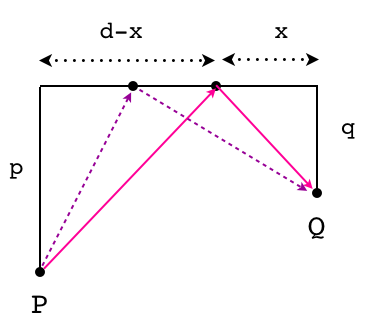
\includegraphics [scale=0.5] {short1.png} \end{center}

Another way to say it is that the angle where we come from $P$ to the river, and the angle by which we leave the river to $Q$ should be equal.

Now for the easy way.

\begin{center} 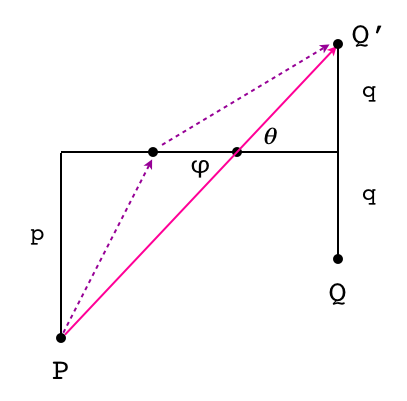
\includegraphics [scale=0.5] {short2.png} \end{center}

We draw a vertical up the same distance $q$ to point $Q'$---the mirror image of $Q$.  Minimizing the distance to $Q'$ is the same problem because it's exactly the same distance.

What's the shortest distance between two points?  A straight line from $P$ to $Q'$.  With a straight line then the two angles $\phi$ and $\theta$ are equal and the similarity of the triangles follows immmediately.

This is a famous result in physics.  It's true for light rays, that when you shine a light from $P$ at a mirror, the light rays arriving at $Q$ come by the shortest path.  The law about the angles being equal is called the "law of reflection" and it was known to Euclid.

Pool players who know nothing about about Euclid know this result, and they use it all the time in making bank shots.

But this is only the beginning.  The general principle is called "least action."

\section*{Snell's Law}

\label{sec:Snells_law}
A variation on the previous problem yields Snell's Law for refraction.

Consider the problem of a light ray passing from $P$ to $Q$, where $P$ is in air, and $Q$ is in a medium like water, with a higher refractive index and lower speed of light.  

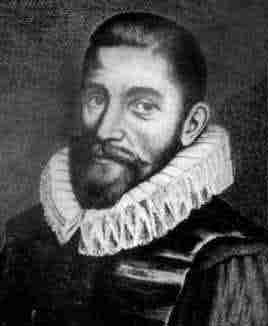
\includegraphics [scale=0.6] {Snell.jpg} 
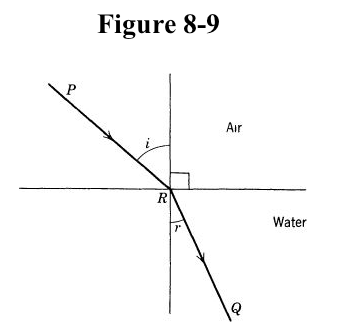
\includegraphics [scale=0.6] {snell_law.png}

The physical principle is that light takes the path of shortest time.  We need to find the $R$ that makes this true.

Suppose the total horizontal distance between $P$ and $Q$ is $d$.  Let $x$ be the horizontal distance from $P$ to $R$, then $d - x$ is the horizontal distance from $R$ to $Q$.  The vertical distances are fixed, let's call them $p$ (for $PR$) and $q$ (for $QR$).

The time taken is the distance divided by the speed.  Let the speed of light in air be $u$ and the speed of light in water be $v$.  There are two segments of the trip:
\[ t_1 = \frac{\sqrt{x^2 + p^2}}{u} \]
\[ t_2 = \frac{\sqrt{(d-x)^2 + q^2}}{v} \]
\[ t = t_1 + t_2 = \frac{\sqrt{x^2 + p^2}}{u} + \frac{\sqrt{(d-x)^2 + q^2}}{v} \]

We have time $t$ as a function of $x$ and we take the first derivative and set it equal to zero:

\[ \frac{x}{u \sqrt{x^2 + p^2}} + \frac{-(d-x)}{v \sqrt{(d-x)^2 + q^2}}  = 0  \]
\[ \frac{x}{u \sqrt{x^2 + p^2}} = \frac{(d-x)}{v \sqrt{(d-x)^2 + q^2}}  \]

Rather than fool with the square roots, notice that
\[ \sqrt{x^2 + p^2} = PR \]
and
\[ \sqrt{(d-x)^2 + q^2} = RQ \]
so
\[ \frac{x}{u \sqrt{x^2 + p^2}} = \frac{(d-x)}{v \sqrt{(d-x)^2 + q^2}}  \]
becomes
\[ \frac{x}{u \ {PR}} = \frac{(d-x)}{v\  {RQ}}  \]

Furthermore $x/PR = \sin \theta_i$ and $(d-x)/RQ = \sin \theta_r$ so
\[ \frac{\sin \theta_i}{u} = \frac{\sin \theta_r}{v}  \]
The sines of the angles for each side of the barrier are in the same ratio as the velocities in the respective medium.
\[ \frac{\sin \theta_i}{\sin \theta_r} = \frac{u}{v}  \]
\[ \sin \theta_r = \frac{v}{u} \ \sin \theta_i \]

Since the speed of light in air is higher than in water $u > v$, $v/u < 1$ which means that $\sin \theta_r < \sin \theta_i$ and thus $\theta_r < \theta_i$.

We can also use the refractive index $n$ which is proportional to the reciprocal of the speed.
\[ \frac{\sin \theta_i}{\sin \theta_r} = \frac{n_r}{n_i}  \]


\end{document}